%%%%%%%%%%%%%%%%%%%%%%%%%%%%%%%%%%%%%%%%%%%%%%%%%%%%%%%%%%%%%%%%%%%%%%%%%%%%%%%%%%%%%%%%
\chapter[Transition Metal Oxides as Kitaev Materials]{Transition Metal Oxides as\linebreak Kitaev Materials}
\label{chapter:TransitionMetalOxides}
%%%%%%%%%%%%%%%%%%%%%%%%%%%%%%%%%%%%%%%%%%%%%%%%%%%%%%%%%%%%%%%%%%%%%%%%%%%%%%%%%%%%%%%%
%
%
Just a few years after Kitaev introduced his exactly solvable honeycomb model, Jackeli and Khaliullin had proposed a physical realization of the model in certain strongly spin-orbit coupled Mott insulators~\cite{JackeliPRL2009}.
In particular, they proposed that $A_2MO_3$ compounds, where $A$ and $M$ are alkali and late transition metal ions, respectively, could realize Kitaev exchange between local $j_{\rm eff} = 1/2$ moments for a certain arrangement of the ligand oxygen ions.

In such a material, the transition metal cations are surrounded by an octahedral cage of oxygen anions.
The crystal electric field resulting from the oxygens splits the degeneracy of the transition metal's partially filled $d$ subshell into an empty high-energy $e_g$ manifold and a low-energy $t_{2g}$ manifold with a single hole.
As the transition metal ions are quite massive, strong spin-orbit coupling further splits the degeneracy of the $t_{2g}$ bands, ultimately yielding a spin-orbit entangled $j_{\rm eff} = 1/2$ moment.
Although the $4d$ and $5d$ orbitals of the transition metal ions are rather extended resulting in a relatively weak on-site Coulomb repulsion, the narrow bandwidth of the $j_{\rm eff} = 1/2$ doublet allows for the formation of a so-called spin-orbit assisted Mott insulator.
Jackeli and Khaliullin showed that for idealized edge-sharing octahedra with inversion symmetry, the superexchange between the transition metal ions due to the oxygen ligands is precisely the Kitaev interaction.

This realization spawned an intense effort to find such Kitaev materials in the laboratory.
While a number of honeycomb materials -- as well as a number of \textit{three-dimensional} variants -- have been found to harbor dominant Kitaev interactions, all of these materials have been observed to exhibit long-range magnetic order at finite temperatures due to the presence of additional exchange interactions.
Despite the observation of magnetic order, it has been argued that at least one of these materials is \textit{proximate} to a Kitaev spin liquid phase and that evidence of fractionalization is seen to occur in certain thermodynamic signatures -- a claim which remains controversial.
The discovery of three-dimensional Kitaev materials has sparked much theoretical interest in three-dimensional Kitaev spin liquids, including the work reported in this thesis.

The remainder of this chapter is structured as follows.
Section~\ref{section:chapter03_CFSO} gives a detailed description of the mechanism by which the spin-orbit assisted Mott insulator forms in the transition metal oxides.
The superexchange mechanism leading to the Kitaev interaction is treated in Section~\ref{section:chapter03_SpinExchange}.
Inclusion of additional exchange interactions is also discussed in this section.
A brief overview of some prominent Kitaev materials in both two- and three-dimensions is given Section~\ref{section:chapter03_Materials}.
Finally, Section~\ref{section:chapter03_Summary} provides a brief summary.


%
%
%%%%%%%%%%%%%%%%%%%%%%%%%%%%%%%%%%%%%%%%%%%%%%%%%%%%%%%%%%%%%%%%%%%%%%%%%%%%%%%%%%%%%%%%
\section{Spin-orbit entangled \texorpdfstring{$J_{\rm eff} = 1/2$}{Jeff=1/2}~Mott insulators}
\label{section:chapter03_CFSO}
%%%%%%%%%%%%%%%%%%%%%%%%%%%%%%%%%%%%%%%%%%%%%%%%%%%%%%%%%%%%%%%%%%%%%%%%%%%%%%%%%%%%%%%%
%
%
%
\begin{figure}[tb]
	\centering
	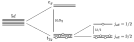
\includegraphics[width=\linewidth]{./chapter03/LevelSplitting.pdf}
	\caption{
		Splitting of $5d$ orbitals by crystal electric field and spin-orbit coupling resulting in $j_{\rm eff} = 1/2$ moment.
	}
	\label{fig:chapter03_LevelSplitting}
\end{figure}
%
In a spherically symmetric potential and without considering the relativistic effect of spin-orbit coupling, the state of an electron in an isolated atom or ion is characterized by the principle quantum number $n = 1, 2, \ldots$, the azimuthal quantum number $l = 0, 1, \ldots, n - 1$, the corresponding magnetic quantum number $m_l \in \{-l, -l+1, \ldots, l\}$ and the electron spin $m_s = \pm 1$, \ie,
%
\begin{equation}
	\ket{\psi_{\rm el}} = \ket{n, l, m_l, m_s}.
\end{equation}
%
Whereas the principle quantum number $n$ dictates the spatial extent of the electronic wave function -- with larger $n$ corresponding to a more delocalized electron -- $l$ and $m_l$ determine the orbital angular momentum and govern the shape of the wave function.
Different values of the orbital angular momentum $l$ correspond to \textit{subshells} of the $n^{\rm th}$ \textit{shell} and the different values of the magnetic quantum number $m_l$ correspond to the different \textit{orbitals}.
The orbitals in a subshell are commonly referred to as $s$-, $p$-, $d$-, or $f$-orbitals, corresponding to orbital angular momentum $l=0, 1, 2, 3$, respectively.
Beyond $l = 3$ the naming continues alphabetically with the exception that there are no $j$-orbitals.
For fixed values of $n$ and $l$, there are a total of $2 \times (2l + 1)$ degenerate states corresponding to the $2l + 1$ allowed values of the magnetic quantum number $m_l$ and the two possible values of the electron spin $m_s$.

This section will discuss the partial lifting of this degeneracy in the context of certain iridate compounds via anisotropic electric potentials -- the so-called \textit{crystal field} -- and by spin-orbit coupling.
For the case of five electrons in a partially filled $d$ subshell, it will be shown that the resulting low-energy description is that of an effective spin-1/2 moment (see Figure~\ref{fig:chapter03_LevelSplitting}).
Furthermore, electronic correlations are seen to localize the effective spin-1/2 degrees of freedom in a Mott insulating state.


%
%
\subsection{Crystal field splitting}
%
%
%
\begin{figure}[tb]
	\centering
	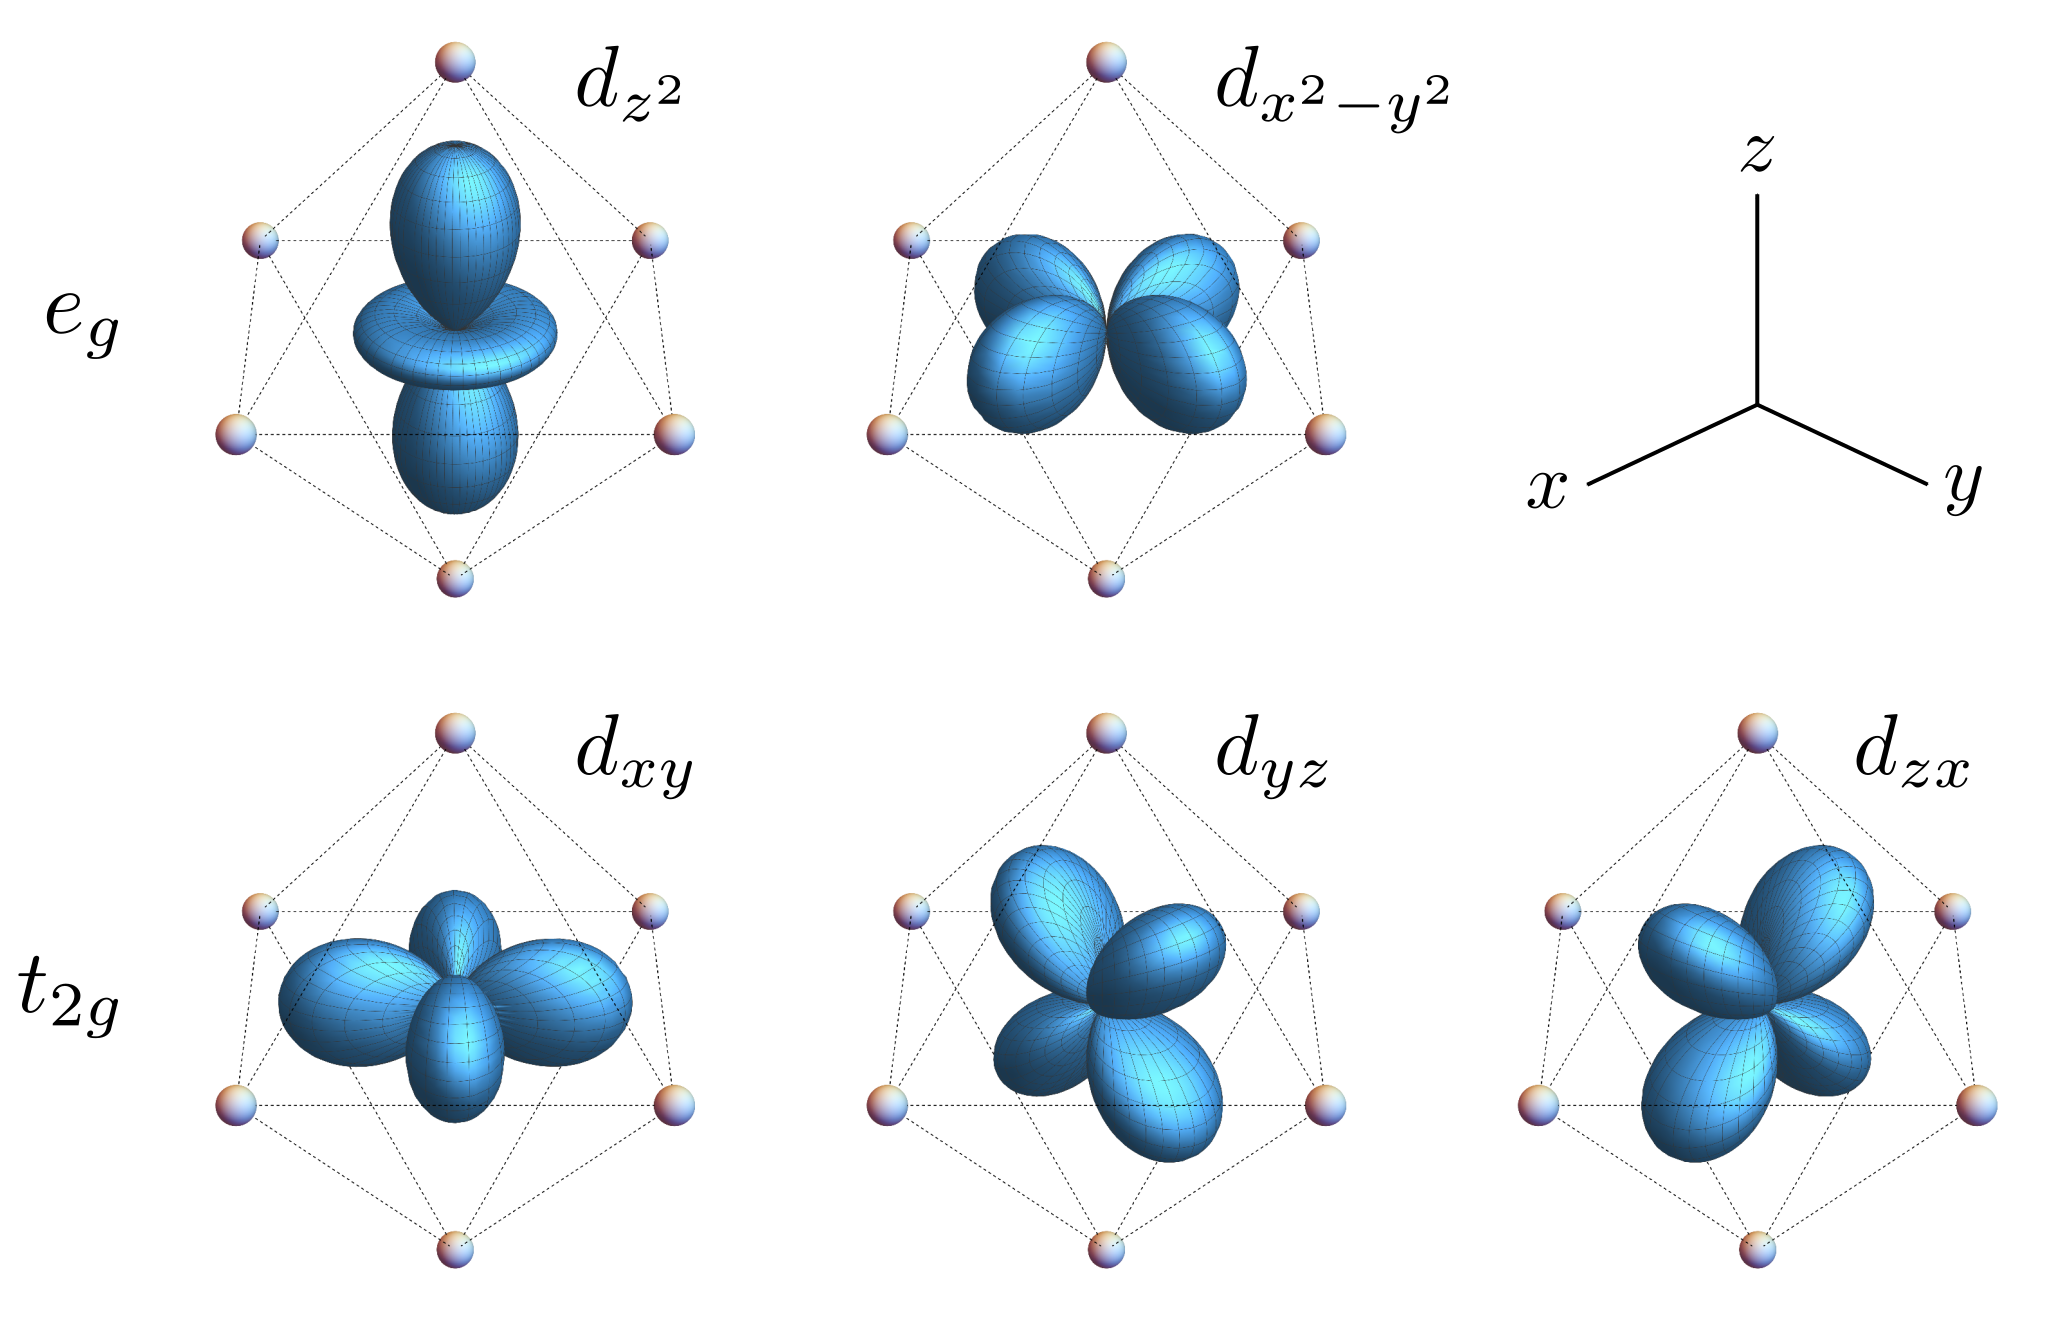
\includegraphics[width=\linewidth]{./chapter03/IridiumOrbitals.pdf}
	\caption{
		Higher energy $e_g$ and lower energy $t_{2g}$ orbitals of a transition metal cation in the center of an octahedral cage of ligand oxygen anions.
		The lobes of the $e_g$ orbitals are extended \textit{toward} the oxygen ligands, whereas the lobes of the $t_{2g}$ orbitals lie \textit{between} the ligands.
	}
	\label{fig:chapter03_SpatialOrbitals}
\end{figure}
%
In, \eg, the iridate materials Ir$^{4+}$ cations are surrounded by an octahedral cage of ligand O$^{2-}$ anions (see Figure~\ref{fig:chapter03_SpatialOrbitals}).
The resulting crystal electric field experienced by the electrons in the iridium atom, thus, exhibits a cubic symmetry.
As the orbital angular momentum determines the shape of the wave function, the cubic anisotropy naturally leads to a splitting of the orbital degeneracy.

In the case of the iridates, the iridium ions have a partially filled 5$d$-subshell.
The $d$-orbitals in an isolated ion have a fivefold degeneracy and may be specified by their total orbital angular momentum $l = 2$ along with their magnetic quantum number $m_l \in \{ 0, \pm 1, \pm 2 \}$ as $\ket{l, m_l}$ (suppressing the principle and spin quantum numbers).
The interaction of the $d$-electrons with the surrounding ions in the crystal, however, leads to a splitting of this degeneracy known as \textit{crystal field splitting}.
The $d$-orbitals are split into a lower-energy $t_{2g}$ triplet and a higher-energy $e_g$ doublet given by~\cite{Ballhausen1962,Griffith1971}
%
\begin{align}
	\begin{matrix*}[l]
		\begin{matrix*}[l]
			\ket{z^2}			\\
			\ket{x^2 - y^2}		
		\end{matrix*}
		&
		\begin{matrix*}[l]
			= \\
			=
		\end{matrix*}
		&
		\begin{matrix*}[l]
			\ket{2, 0} \\
			\frac{1}{\sqrt{2}} (\ket{2, 2} + \ket{2, -2})
		\end{matrix*}
		&
		\left.
		\begin{matrix*}[l]
			\\ \\
		\end{matrix*}
		\right\}~e_g~{\rm orbitals} \nonumber\\
		\nonumber\\
		\begin{matrix*}[l]
			\ket{xy}	\\
			\ket{yz}	\\
			\ket{zx}	
		\end{matrix*}
		&
		\begin{matrix*}[l]
			= \\
			= \\
			=
		\end{matrix*}
		&
		\begin{matrix*}[l]
			-\frac{i}{\sqrt{2}} (\ket{2, 2} - \ket{2, -2}) \\
			\phantom{-}\frac{i}{\sqrt{2}} (\ket{2, 1} + \ket{2, -1}) \\
			-\frac{1}{\sqrt{2}} (\ket{2, 1} - \ket{2, -1})
		\end{matrix*}
		&
		\left.
		\begin{matrix*}[l]
			\\ \\ \\
		\end{matrix*}
		\right\}~t_{2g}~{\rm orbitals}.
	\end{matrix*}
\end{align}
%

Referring to the above orbitals pictured in Figure~\ref{fig:chapter03_SpatialOrbitals}, one can understand this splitting from a purely geometric perspective.
Whereas the lobes of the $e_g$ orbitals are extended \textit{toward} the oxygen ligands, the lobes of the $t_{2g}$ orbitals lie \textit{between} the ligands.
The Coulomb interaction, thus, works to raise the energy of the $e_g$ orbitals relative to the $t_{2g}$ orbitals.
This contribution to the crystal field splitting is known as the \textit{point charge contribution}.
Additionally, one should consider the effects of hybridization of the $d$-orbitals of the iridium ions with the $p$-orbitals of the surrounding ligands.
Such hybridization is stronger for the $e_g$ orbitals than for the $t_{2g}$ orbitals, resulting in a level splitting.
Although the splitting due to hybridization tends to be stronger than the point charge contribution, they both result in the same qualitative behavior and, thus, the point charge picture is generally invoked to provide a simpler illustration of the crystal field splitting mechanism~\cite{Khomskii2014}.
The resulting energy splitting $\Delta_{CF}$ is often denoted as $10~Dq$ for historical reasons~\cite{SchlappPR1932} and is typically on the order of 2-3 eV~\cite{Maekawa2004}.


%
%
\subsection{Spin-orbit coupling and electronic correlations}
%
%
When spin-orbit coupling is included as $\op{H}_{SOC} = \lambda \op{\bm{L}} \cdot \op{\bS}$, the orbital and spin angular momenta no longer correspond to good quantum numbers and are instead combined to form the total angular momentum operator $\op{\bm{J}} = \op{\bm{L}} + \op{\bS}$.
The new quantum numbers are the total angular momentum $j \in \{|l - s|, |l - s| + 1, \ldots, l + s\}$ and its projection to the $z$-axis $m_j \in \{-j, -j + 1, \ldots, j\}$.
For the lighter $3d$ transition metals, the spin-orbit coupling is not very strong, however, for the heavier $4d$ and $5d$ compounds its effects become pronounced.
Experimental data suggests that the strength of spin-orbit coupling for $5d$ Ir$^{4+}$ ions is $\lambda \sim 380$ meV~\cite{SchirmerJPC1984}.

In order to discuss the effects of $\op{H}_{SOC}$ in the iridates, it is convenient to change bases once again within the $t_{2g}$ triplet.
Projected down to the $t_{2g}$ subspace, the vector components of the orbital angular momentum operator $\op{\bm{L}}$ read
%
\begin{align}
	\begin{matrix*}[l]
		L^x_{t_{2g}} &= \frac{i}{\sqrt{2}}
			\begin{pmatrix}
				0	&	1	&	0	\\
				-1	&	0	&	1	\\
				0	&	-1	&	0
			\end{pmatrix},
		&
		L^y_{t_{2g}} &= \frac{1}{\sqrt{2}}
			\begin{pmatrix}
				0	&	1	&	0	\\
				1	&	0	&	1	\\
				0	&	1	&	0
			\end{pmatrix},
		&
		L^z_{t_{2g}} &=
			\begin{pmatrix}
				-1	&	0	&	0	\\
				0	&	0	&	0	\\
				0	&	0	&	1	
			\end{pmatrix}
	\end{matrix*}
\end{align}
%
in a basis chosen to diagonalize $L^z_{t_{2g}}$.
The above components satisfy the algebraic relations
%
\begin{equation}
	[L^{\alpha}_{t_{2g}}, L^{\beta}_{t_{2g}}] = -i \epsilon_{\alpha\beta\gamma} L^{\gamma}_{t_{2g}}.
\end{equation}
%
It is convenient to define an effective angular momentum operator $\op{\bm{L}}_{\rm eff} = -\op{\bm{L}}_{t_{2g}}$ acting on this subspace, the components of which are now easily seen to satisfy the usual angular momentum algebra~\cite{AbragamPRSL1951}.
The eigenstates of $L^z_{\rm eff}$, thus, furnish an $l_{\rm eff} = 1$ representation of the $t_{2g}$ subspace and may be expressed explicitly as
%
\begin{equation}
	\begin{matrix*}[l]
	\ket{l_{\rm eff} = 1, m_{l_{\rm eff}} = 1}	& = \phantom{-}\frac{1}{\sqrt{2}} (\ket{zx} - i \ket{yz}), \\
	&\\
	\ket{l_{\rm eff} = 1, m_{l_{\rm eff}} = 0}	& = \phantom{-}\ket{xy}, \\
	&\\
	\ket{l_{\rm eff} = 1, m_{l_{\rm eff}} = -1}	& = -\frac{1}{\sqrt{2}} (\ket{xz} + i \ket{yz}).
	\end{matrix*}
	\label{eq:chapter03_OrbitalsLeff}
\end{equation}
%

When projected down to the $t_{2g}$ subspace, the spin-orbit coupling interaction may be written in terms of this effective angular momentum as $\op{H}_{L_{\rm eff} S} = -\lambda \op{\bm{L}}_{\rm eff} \cdot \op{\bS}$, describing the coupling of spin to an effective angular momentum $l_{\rm eff} = 1$ with an overall minus sign.
In the absence of this spin-orbit coupling term, there is a sixfold degeneracy of the $t_{2g}$ orbitals when accounting for the electron spin.
The interaction, however, further splits this degeneracy to a high-energy $j_{\rm eff} = 1/2$ doublet and a low-energy $j_{\rm eff} = 3/2$ quadruplet with an energy difference of $\Delta_{SOC} = 3\lambda/2$, where $\op{\bm J}_{\rm eff} = \op{\bm{L}}_{\rm eff} + \op{\bS}$.
Typically, the spin-orbit interaction would yield higher energies for larger values of $j$, however, as the effective orbital angular momentum $\op{\bm{L}}_{\rm eff}$ changed the overall sign of the spin-orbit interaction within the $t_{2g}$ triplet, the splitting is reversed.

As mentioned above, the iridium cations are in the Ir$^{4+}$ oxidation state,  indicating a total of five valence electrons in the $5d$ subshell.
In the case of an isolated ion, Hund's rules -- which seek to minimize the Coulomb repulsion between electrons on the same ion -- would dictate that all five electrons have the same spin and occupy different $d$ orbitals.
For small values of the crystal field splitting $\Delta_{CF}$ as in the lighter $3d$ transition metal oxides, this would still hold true yielding the \textit{high-spin state}~\cite{Khomskii2014}.
However, as the $5d$ orbitals in the iridates are spatially very extended, $\Delta_{CF}$ tends to be much larger than the Hund's coupling and the \textit{low-spin state}, with all valence electrons in the $t_{2g}$ orbitals, is favored.
After including the spin-orbit coupling, one finds that the $j_{\rm eff} = 3/2$ quadruplet is completely full, leaving a half-filled $j_{\rm eff} = 1/2$ doublet.
Although the on-site Coulomb repulsion $U$ is not very large in the 5$d$ orbitals due to them being very extended, the bandwidth of the $j_{\rm eff} = 1/2$ doublet is very small and, thus, even a small $U$ leads to the opening of a Mott gap.
The ultimate result of this interplay of crystal field effects, spin-orbit coupling and electronic correlations is that the iridate materials are Mott insulators with localized effective "spin"-1/2 degrees of freedom~\cite{KimPRL2008,KimSci2009}.


%
%
%%%%%%%%%%%%%%%%%%%%%%%%%%%%%%%%%%%%%%%%%%%%%%%%%%%%%%%%%%%%%%%%%%%%%%%%%%%%%%%%%%%%%%%%
\section{Spin exchange mechanism}
\label{section:chapter03_SpinExchange}
%%%%%%%%%%%%%%%%%%%%%%%%%%%%%%%%%%%%%%%%%%%%%%%%%%%%%%%%%%%%%%%%%%%%%%%%%%%%%%%%%%%%%%%%
%
%
\subsection{Idealized Kitaev interaction}
%
%
%
\begin{figure}[tb]
	\centering
	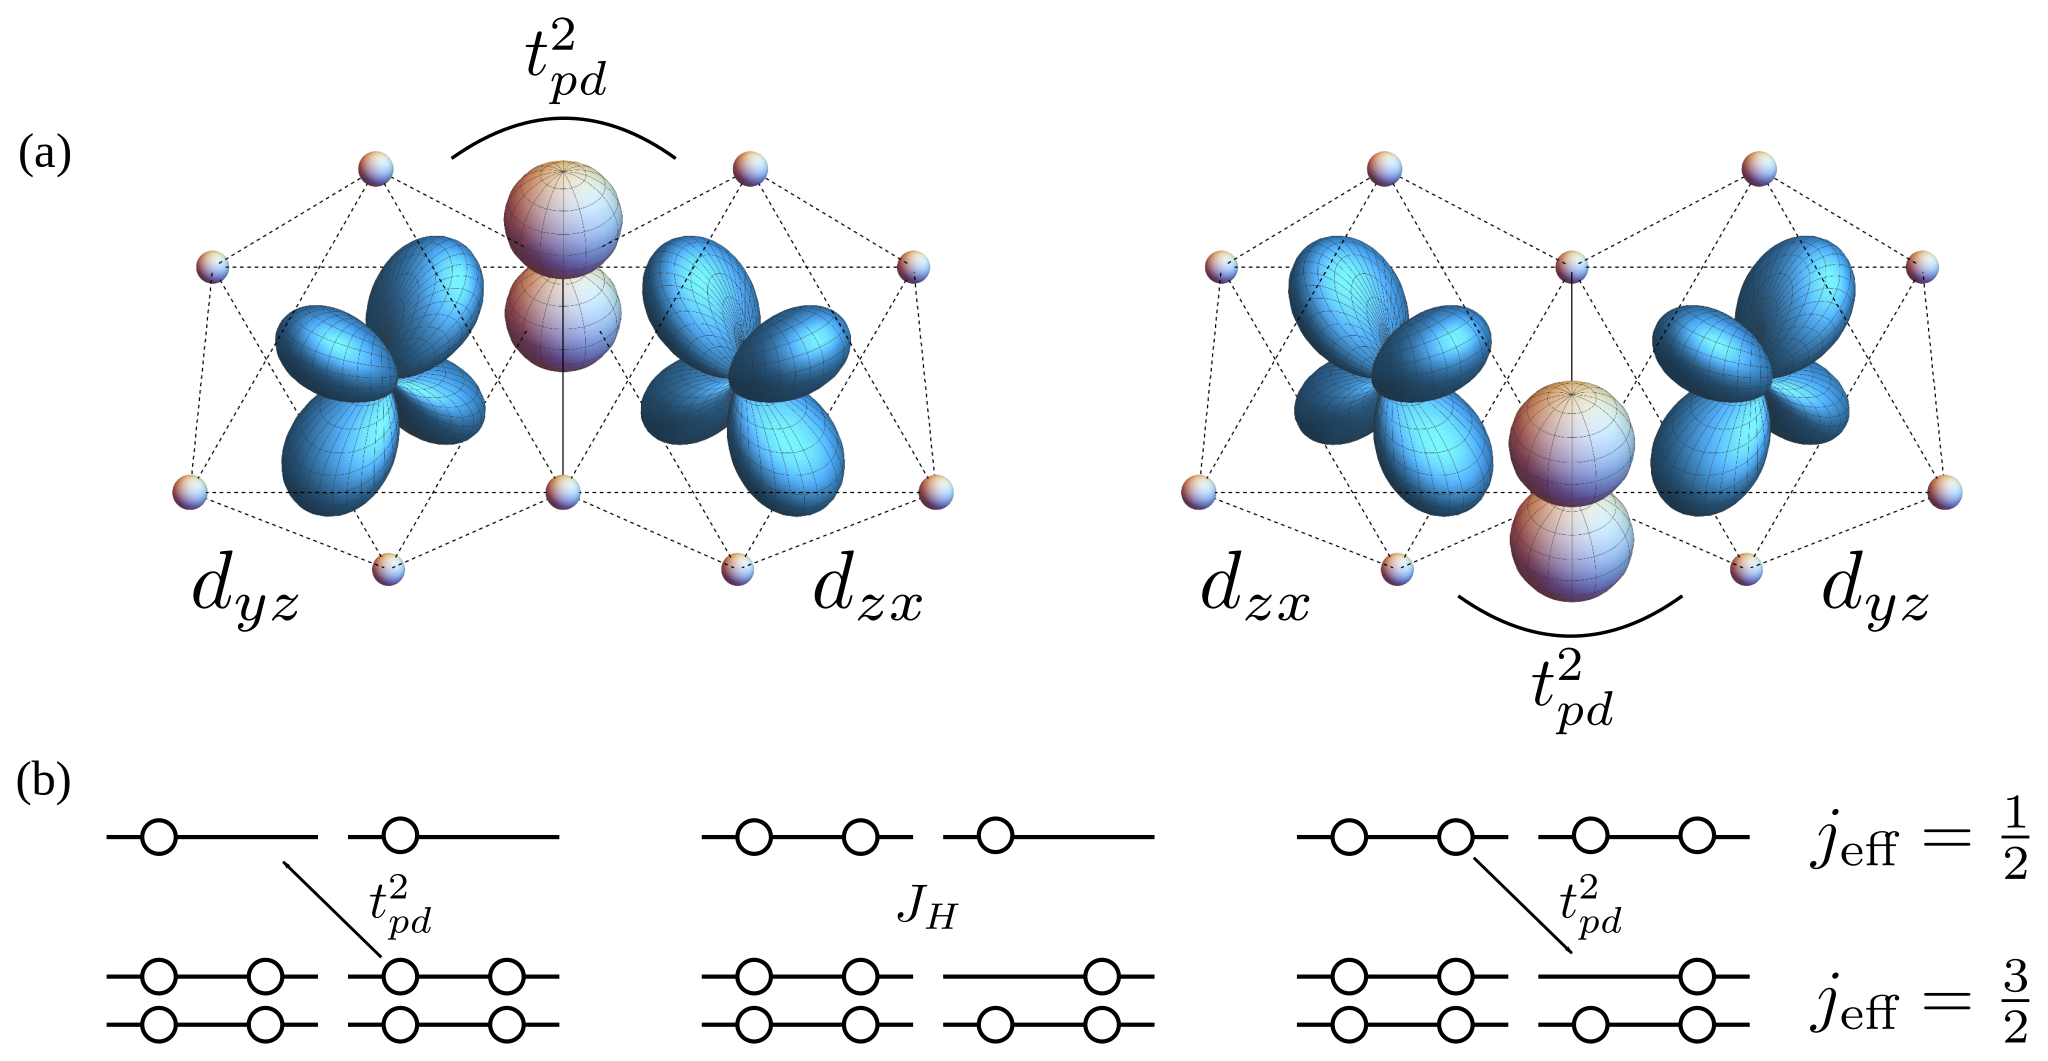
\includegraphics[width=\linewidth]{./chapter03/PerturbationTheory.pdf}
	\caption{
		(a) Two distinct 90$^{\circ}$ exchange paths for a hole to hop from the iridium site on the left to the iridium site on the right via an oxygen ligand.
		(b) Schematic of the exchange of a hole from the $j_{\rm eff} = 1/2$ state of the iridium ion on the left to a $j_{\rm eff} = 3/2$ state of the iridium ion on the right and back again.
	}
	\label{fig:chapter03_ExchangePaths}
\end{figure}
%
For the Mott insulating $5d$ iridates described above, a "spin" Hamiltonian may be derived via perturbation theory describing their interaction via the 90$^{\circ}$ exchange paths shown in Figure~\ref{fig:chapter03_ExchangePaths}~(a).
Here, the spin degrees of freedom correspond to the spin-orbit entangled $j_{\rm eff} = 1/2$ moments described above.
In this context, it will be simpler to think of there being a single hole at each iridium ion.
The superexchange mechanism originally considered by Jackeli and Khaliullin~\cite{JackeliPRL2009} allowed for hopping of holes between neighboring iridium ions via the oxygen ligands.
No direct $d-d$ hopping between iridium ions was considered, only hopping back and forth using the \textit{same} ligand was allowed, \ie, no cyclic exchange of holes around the Ir$_2$O$_2$ plaquette, and processes involving two holes on the same ligand were ignored due to strong Coulomb repulsion on the oxygen ions.
For the edge-sharing octahedra shown in Figure~\ref{fig:chapter03_ExchangePaths}~(a), a hole may hop from a $d_{zx}$-orbital to a $p_z$-orbital to a $d_{yz}$-orbital and back, or vice versa. 
In general, the active orbitals depend on the direction of the Ir-O-Ir exchange paths due to the anisotropic nature of the spin-orbit entangled moments.

For holes hopping between $j_{\rm eff} = 1/2$ orbitals it is clear that the resulting interaction is of the antiferromagnetic Heisenberg type $J \bS_i \cdot \bS_j$, where $J \sim t_{pd}^4 / U_d^2$, $t_{pd}$ is the hopping amplitude between $d$ and $p$ orbitals on the iridium and oxygen ions, respectively, $U_d$ is the local Coulomb repulsion on the iridium ions and $\bS_{i/j}$ are the effective spins living on neighboring iridium ions.
As can be seen in Figure~\ref{fig:chapter03_ExchangePaths}~(a), however, there are two such exchange paths -- one via the "upper" oxygen and one via the "lower" oxygen.
Jackeli and Khaliullin showed that the contributions from these two paths interfere destructively and cancel one another exactly.

There remains, however, the possibility for a hole to hop from the $j_{\rm eff} = 1/2$ doublet at one iridium site to the $j_{\rm eff} = 3/2$ quadruplet at the other site and then back (see Figure~\ref{fig:chapter03_ExchangePaths}~(b)).
In fact, the only relevant hopping is between $j_{\rm eff} = 1/2$ states and $m_{j_{\rm eff}} = \pm 3/2$ states~\cite{WinterJOP2017}.
Such processes ultimately generate a ferromagnetic interaction which does not affect the local arrangement of effective spins, \ie, it is of ferromagnetic Ising form $-J_K S_i^z S_j^z$, where $J_K \sim t_{pd}^4 J_H / U_d^2$ with the Hund's coupling $J_H$ acting between the $j_{\rm eff} = 1/2$ and excited $j_{\rm eff} = 3/2$ moments.
For other bond orientations with active $p_x$ or $p_y$ oxygen orbitals, the resulting anisotropic interaction instead couples the $x$- or $y$-components of the local moments, respectively.
For the honeycomb iridate compounds A$_2$IrO$_3$ to be discussed below, each iridium ion interacts with three neighbors through three distinct pairs of exchange paths (see Figure~\ref{fig:chapter03_HoneycombOctahedra}) and the resulting exchange produces exactly the Kitaev Hamiltonian,
%
\begin{equation}
	\op{H}_{\rm ex} = -J_K \sum_{\avg{i,j}_{\gamma}} S_i^{\gamma} S_j^{\gamma},
\end{equation}
%
where $\gamma$ is determined by the active $p$ orbital responsible for the superexchange between the neighboring $j_{\rm eff} = 1/2$ moments.
%
\begin{figure}[tb]
	\centering
	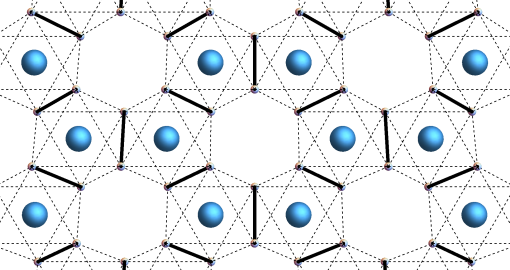
\includegraphics[width=0.8\linewidth]{./chapter03/HoneycombOctahedra.pdf}
	\caption{
		Honeycomb arrangement of iridium ions situated at the centers of edge-sharing oxygen octahedra.
		Shared edges responsible for Kitaev exchange between nearest neighbor iridium ions are marked with solid black lines.
	}
	\label{fig:chapter03_HoneycombOctahedra}
\end{figure}
%


%
%
\subsection{Additional exchange terms}
%
%
While the above mechanism for Kitaev exchange in a honeycomb iridate compound is elegant, in order to realistically discuss such a material a number of other effects should be considered.
To begin with, for compounds consisting of the heavier $4d$ and $5d$ transition metals, direct overlap of $d$ orbitals from neighboring ions may be significant.
As already mentioned, the analysis of the last section ignores the effects of direct $d-d$ hopping between neighboring iridium ions as well as cyclic exchange of holes around an Ir$_2$O$_2$ plaquette and the possibility of two holes simultaneously occupying an oxygen ion.
While the overlap of $d_{xy}$ orbitals from neighboring iridium ions leads to the usual antiferromagnetic Heisenberg exchange, the latter processes contribute both Heisenberg exchange as well as the anisotropic Kitaev interaction, yielding the effective model~\cite{ChaloupkaPRL2010}
%
\begin{equation}
	\op{H} = J \sum_{\avg{i,j}} \bS_i \cdot \bS_j - J_K \sum_{\avg{i,j}_{\gamma}} S^{\gamma}_i S^{\gamma}_j.
\end{equation}
%
In fact, allowing for exchange via \textit{all} $d$ orbitals introduces additional spin interactions leading to an effective Hamiltonian~\cite{WinterPRB2016,RauPRL2014}
%
\begin{align}
	\op{H} 	&= \sum_{\substack{\avg{i,j}_{\gamma}\\ \alpha,\beta \neq \gamma}} \Big(J_{ij} \bS_i \cdot \bS_j + K_{ij} S^{\gamma}_i S^{\gamma}_j + \Gamma_{ij} (S^{\alpha}_i S^{\beta}_j + S^{\beta}_i S^{\alpha}_j) \nonumber\\
			&\qquad\qquad+ \Gamma'_{ij} (S^{\gamma}_i S^{\alpha}_j + S^{\gamma}_i S^{\beta}_j + S^{\alpha}_i S^{\gamma}_j + S^{\beta}_i S^{\gamma}_j)\Big).
\end{align}
%

The $\Gamma'$ term above actually vanishes for cubic symmetry, however, real materials typically lack such perfect symmetry and tend to exhibit a trigonal distortion of the ligand octahedra~\cite{WinterJOP2017}.
Rather than producing local spin-orbit entangled $j_{\rm eff} = 1/2$ moments, such a distorted crystal field splits the degeneracy of the $t_{2g}$ orbitals and results in local moments with a different mixture of spin and orbital character.
For significantly small distortions which only partially quench the orbital angular momentum, additional anisotropic exchange terms are present, \eg, the $\Gamma'$ term above.
However, for distortions which completely lift the $t_{2g}$ degeneracy the local moments are pure $s = 1/2$ moments and exhibit nearly isotropic Heisenberg exchange~\cite{WinterJOP2017}.
Additionally, a finite Dzyaloshinskii-Moriya interaction $\bm{D}\cdot(\bS_i \times \bS_j)$ is permitted for \textit{second}-nearest neighbors in all Kitaev candidate lattices as well as certain nearest-neighbor bonds in the 3D materials~\cite{WinterPRB2016}.


%
%
%%%%%%%%%%%%%%%%%%%%%%%%%%%%%%%%%%%%%%%%%%%%%%%%%%%%%%%%%%%%%%%%%%%%%%%%%%%%%%%%%%%%%%%%
\section{Kitaev materials}
\label{section:chapter03_Materials}
%%%%%%%%%%%%%%%%%%%%%%%%%%%%%%%%%%%%%%%%%%%%%%%%%%%%%%%%%%%%%%%%%%%%%%%%%%%%%%%%%%%%%%%%
%
%
This section provides a brief overview of the two-dimensional honeycomb materials, namely the iridates Na$_2$IrO$_3$ and $\alpha$-Li$_2$IrO$_3$ and the honeycomb ruthenate RuCl$_3$, as well as the three-dimensional hyperhoneycomb and stripy-honeycomb iridates $\beta$-Li$_2$IrO$_3$ and $\gamma$-Li$_2$IrO$_3$, respectively.


%
%
%%%%%%%%%%%%%%%%%%%%%%%%%%%%%%%%%%%%%%%%%%%%%%%%%%%%%%%%%%%%%%%%%%%%%%%%%%%%%%%%%%%%%%%%
\subsubsection{Honeycomb Na$_2$IrO$_3$}
%%%%%%%%%%%%%%%%%%%%%%%%%%%%%%%%%%%%%%%%%%%%%%%%%%%%%%%%%%%%%%%%%%%%%%%%%%%%%%%%%%%%%%%%
%
%
The first Kitaev material extensively studied at low temperatures was the honeycomb iridate Na$_2$IrO$_3$~\cite{SinghPRB2010}.
This material, as well as its counterpart $\alpha$-Li$_2$IrO$_3$ discussed below, is composed of weakly coupled honeycomb planes of oxygen octahedra with iridium ions at their centers.
The compound has been identified as a Mott insulator via electrical resistivity~\cite{SinghPRB2010} and ARPES measurements which indicate nearly dispersionless $t_{2g}$ bands~\cite{CominPRL2012,AlidoustPRB2016,LuepkePRB2015}.
Measurements of the crystal field splitting using resonant inelastic x-ray scattering confirm a spin-orbit entangled $j_{\rm eff} = 1/2$ picture~\cite{GretarssonPRL2013}.

The  material was found to exhibit magnetic order below a N\'eel temperature of $T_N = 13 - 18$ K, where it has been observed to develop a zigzag order~\cite{SinghPRB2010,ChoiPRL2012,YePRB2012,LiuPRB2011}.
Although direct evidence of a dominant Kitaev exchange has been provided by diffuse resonant x-ray scattering~\cite{BarreiroNatPhys2015}, other exchange terms have been estimated to be between 10-30\% of the nearest-neighbor Kitaev exchange~\cite{KatukuriNJP2014,WinterPRB2016,KimchiPRB2011,ChoiPRL2012,ChaloupkaPRB2016}.
Despite Kitaev interactions dominating in agreement with the picture set forth by Jackeli and Khaliullin, additional exchange interactions work to stabilize the zigzag order at low temperatures.


%
%
%%%%%%%%%%%%%%%%%%%%%%%%%%%%%%%%%%%%%%%%%%%%%%%%%%%%%%%%%%%%%%%%%%%%%%%%%%%%%%%%%%%%%%%%
\subsubsection{Honeycomb $\alpha$-Li$_2$IrO$_3$}
%%%%%%%%%%%%%%%%%%%%%%%%%%%%%%%%%%%%%%%%%%%%%%%%%%%%%%%%%%%%%%%%%%%%%%%%%%%%%%%%%%%%%%%%
%
%
Like its counterpart above, $\alpha$-Li$_2$IrO$_3$ has been established as a Mott insulating honeycomb material with dominant Kitaev exchange interactions~\cite{KobayashiJMC2003,SinghPRL2012}.
Evidence of spin-orbit entangled $j_{\rm eff} = 1/2$ moments has been obtained through measurements of crystal field splitting using resonant inelastic x-ray scattering~\cite{GretarssonPRL2013}.
$\alpha$-Li$_2$IrO$_3$ also develops long-range magnetic order below a  N\'eel temperature of $T_N = 15$ K, where it hosts incommensurate counter-rotating spirals~\cite{SinghPRL2012,WilliamsPRB2016}.
The formation of this incommensurate state also requires a large Kitaev exchange~\cite{WilliamsPRB2016}, however, the role of other exchange interactions in this material remains unclear~\cite{WinterJOP2017}.


%
%
%%%%%%%%%%%%%%%%%%%%%%%%%%%%%%%%%%%%%%%%%%%%%%%%%%%%%%%%%%%%%%%%%%%%%%%%%%%%%%%%%%%%%%%%
\subsubsection{Honeycomb $\alpha$-RuCl$_3$}
%%%%%%%%%%%%%%%%%%%%%%%%%%%%%%%%%%%%%%%%%%%%%%%%%%%%%%%%%%%%%%%%%%%%%%%%%%%%%%%%%%%%%%%%
%
%
More recently, much interest has been expressed in the $4d$ compound $\alpha$-RuCl$_3$ as a possible \textit{proximate} Kitaev spin liquid material.
The chlorine octahedra exhibit a nearly perfect cubic symmetry with minimal trigonal distortion and the ruthenium ions form a nearly perfect honeycomb lattice~\cite{TrebstARXIV2017}.
The material has been identified as a Mott insulator via resistivity and photoconductivity measurements~\cite{BinottoPSS1971} as well as photoemission~\cite{ZhouPRB2016,KoitzschPRL2016,SinnSciRep2016} and inverse photoemission experiments~\cite{SinnSciRep2016}.
Spin-orbit coupling plays less of a role than in the iridates due to the lighter $4d$ ruthenium ions~\cite{JohnsonPRB2015}, however, indications of $j_{\rm eff} = 1/2$ moments have been given by x-ray absorption spectroscopy~\cite{PlumbPRB2014,LampenPRL2017}, electron energy loss spectroscopy~\cite{KoitzschPRL2016} and low-energy optical response~\cite{SandilandsPRB2016}.

High quality single crystals of $\alpha$-RuCl$_3$ have been observed to exhibit a transition at $T_N = 7$ K~\cite{BanerjeeScience2017} to a zigzag ordered phase~\cite{JohnsonPRB2015,SearsPRB2015,BanerjeeNatMat2016}.
Raman scattering measurements have revealed a continuum of magnetic excitations well above the ordering temperature~\cite{SandilandsPRL2015} reminiscent of predictions for a pure Kitaev spin liquid phase~\cite{KnollePRL2014}.
This excitation continuum is further supported by inelastic neutron scattering experiments~\cite{BanerjeeScience2017,RanPRL2017}.
It has been suggested~\cite{NasuNatPhys2016} that the temperature dependence of the continuum implies the existence of fractionalized fermionic excitations and claims that $\alpha$-RuCl$_3$ is in close proximity to a Kitaev spin liquid phase.
However, it has been pointed out that these observations may also be explained by off-diagonal exchange resulting in the decay of magnons into a broad continuum of multi-magnon states~\cite{WinterNatComm2017}.
This conclusion is independent of proximity to a Kitaev spin liquid state and demonstrates that such proximity is not necessarily implied by the data.


%
%
%%%%%%%%%%%%%%%%%%%%%%%%%%%%%%%%%%%%%%%%%%%%%%%%%%%%%%%%%%%%%%%%%%%%%%%%%%%%%%%%%%%%%%%%
\subsubsection{Hyperhoneycomb $\beta$-Li$_2$IrO$_3$ and stripy-honeycomb $\gamma$-Li$_2$IrO$_3$}
%%%%%%%%%%%%%%%%%%%%%%%%%%%%%%%%%%%%%%%%%%%%%%%%%%%%%%%%%%%%%%%%%%%%%%%%%%%%%%%%%%%%%%%%
%
%
The discovery of the three-dimensional Li$_2$IrO$_3$ polymorphs on the tricoordinated honeycomb and stripy-honeycomb lattices in the form of $\beta$-Li$_2$IrO$_3$~\cite{TakayamaPRL2015} and $\gamma$-Li$_2$IrO$_3$~\cite{ModicNatComm2014}, respectively, drove much of the theoretical interest in three-dimensional Kitaev spin liquids -- including the work reported in this thesis.
Both materials have been shown to be Mott insulators via DC resistivity measurements~\cite{ModicNatComm2014,TakayamaPRL2015}.
\textit{Ab initio} estimates suggest crystal field splitting in the $\beta$ phase to be on par with the honeycomb $\alpha$ phase~\cite{KatukuriSP2016,KimEPL2015}, whereas estimates for trigonal field terms in the $\gamma$ phase are much larger~\cite{WinterJOP2017}.

Both the $\beta$ and $\gamma$ phases exhibit magnetically ordered incommensurate counter-rotating spiral phases below $T_N = 37$ K~\cite{BiffinPRB2014,TakayamaPRL2015} and $T_N = 39.5$ K~\cite{ModicNatComm2014,BiffinPRL2014}, respectively.
Just as in the $\alpha$ phase, the magnetic order of the $\beta$ and $\gamma$ phases leaves a lot of room for interpretation of the exchange interactions.
Both phases can be reproduced with a Heisenberg-Kitaev model with an additional Ising anisotropy~\cite{KimchiPRB2014,KimchiPRB2015}.
However, they have also been shown to be consistent with a nearest-neighbor $J-K-\Gamma$ model~\cite{KimEPL2015,LeePRB2015}.
\textit{Ab initio} studies of the $\beta$ phase further support the $J-K-\Gamma$ picture~\cite{KatukuriSP2016,KimPRB2016,KimEPL2015}, however, it has also been suggested that longer-range interactions play an important role in these materials~\cite{KatukuriSP2016}.


%
%
%%%%%%%%%%%%%%%%%%%%%%%%%%%%%%%%%%%%%%%%%%%%%%%%%%%%%%%%%%%%%%%%%%%%%%%%%%%%%%%%%%%%%%%%
\section{Summary}
\label{section:chapter03_Summary}
%%%%%%%%%%%%%%%%%%%%%%%%%%%%%%%%%%%%%%%%%%%%%%%%%%%%%%%%%%%%%%%%%%%%%%%%%%%%%%%%%%%%%%%%
%
%
This chapter focused on the solid state realization of Kitaev's honeycomb model in certain spin-orbit assisted Mott insulating transition metal oxides.
It was shown how the interplay of strong crystal field effects and strong spin-orbit coupling in such materials results in the splitting of spin and orbital degeneracies to yield a $j_{\rm eff} = 1/2$ degree of freedom.
Due to the narrow bandwidth of the $j_{\rm eff} = 1/2$ doublet, even a relatively weak on-site Coulomb repulsion results in a local moment picture.
The mechanism of ligand-assisted superexchange was discussed which Jackeli and Khaliullin put forth to predict Kitaev interactions in these materials.
Additional magnetic exchange terms were also discussed, the inclusion of which are necessary for a realistic description of the Kitaev materials.
A brief discussion of the relevant two- and three-dimensional materials revealed that these other exchange mechanisms lead to long-range magnetic order in all of the Kitaev materials discovered so far.

It should be mentioned that there have been other proposals for engineering solid state incarnations of Kitaev physics.
In 2017, the Oshikawa group proposed designing Kitaev materials in metal-organic-frameworks (MOF)~\cite{MasahikoPRL2017}.
In an MOF, rather than the edges of ligand octahedra being shared \textit{directly}, additional organic ligands such as $({\rm C}_2{\rm O}_4)^{2-}$ connect the edges of neighboring octahedra.
The idea is that the electron density of the organic ligands screens the wave functions of the metal ions, thereby reducing the direct $d-d$ hopping that leads to most of the other \textit{non}-Kitaev exchange interactions.
Very recently, it has been proposed that Kitaev physics may also be observed in the rare earth magnets with $4f$ rather than $4d/5d$ electrons~\cite{LiPRB2017,LuoARXIV2019}.